%celine.craye@ensta-paristech.fr

\documentclass[12pt]{article}
\usepackage[paper=a4paper,dvips,top=2.5cm,left=2.5cm,right=2.5cm,
    foot=2cm,bottom=2.5cm]{geometry}
\usepackage[utf8]{inputenc}
\usepackage{lipsum}
\usepackage{graphicx}
\usepackage{caption}
\usepackage{subcaption}
\usepackage{amsmath}
\usepackage{gensymb}
\usepackage{listings}
\lstset{language=C++}

\begin{document}
\setlipsumdefault{1-10}
\tableofcontents
% %%%%%%%%%%%%%%%%%%%%%%%%%%%%%%%%%%%%%%%%%%%%%%%%%%%%%%%%%%%%%%%
% %%%%%%%%%%%%%%%%%%%%%REMERCIEMENTS
% %%%%%%%%%%%%%%%%%%%%%%%%%%%%%%%%%%%%%%%%%%%%%%%%%%%%%%%%%%%%%%%
% \section{Remerciement}
% Je remercie....
% \pagebreak
% %%%%%%%%%%%%%%%%%%%%%%%%%%%%%%%%%%%%%%%%%%%%%%%%%%%%%%%%%%%%%%%
% %%%%%%%%%%%%%%%%%%%%%ENTREPRISE
% %%%%%%%%%%%%%%%%%%%%%%%%%%%%%%%%%%%%%%%%%%%%%%%%%%%%%%%%%%%%%%%
% \section{Entreprise}
% Thales...
% \pagebreak
% %%%%%%%%%%%%%%%%%%%%%%%%%%%%%%%%%%%%%%%%%%%%%%%%%%%%%%%%%%%%%%%
% %%%%%%%%%%%%%%%%%%%%%INTRO
% %%%%%%%%%%%%%%%%%%%%%%%%%%%%%%%%%%%%%%%%%%%%%%%%%%%%%%%%%%%%%%%
\pagebreak
\section{Remerciements}
Je souhaiterais remercier toutes les personnes qui m'ont apporté leur aide lors de ce stage.\\
M\textsuperscript{r} Jean-François GOUDOU, mon superviseur au sein de l'entreprise, pour avoir permis de mettre en place le sujet, et pour sa ???guidance??? au long de celui-çi.\\
\\
M\textsuperscript{lle} Céline CRAYE, pour ses nombreux conseils et participations à la réalisation de ce projet.\\
\\
Tous les membres du laboratoire Theresis/Vision Lab dont les idées m'ont aidé à \\
\\
Elodie EHEM et Edith DE BENGY pour la gestion des procédures administratives nécessaire à ce stage ainsi que le service des stages de l'INSA.\\
\\
Enfin Murielle PRESSIGOUT, ma tutrice au sein de l'INSA pour avoir valider ce sujet et pour la lecture de ce rapport et l'évaluation de mon projet de fin d'étude.
\pagebreak
\section{Introduction}
\subsection{Présentation de Thales}
\subsubsection{Le groupe}
Présent dans 56 pays avec plus de 62 000 salariés, Thales est un des leaders mondiaux des systèmes d'information critiques sur les marchés de l'aéronautique, de l'espace, du transport, de la défense et de la sécurité.\\
Avec environ 14 milliards d'euros de revenus en 2015, le capital du groupe est détenu à 26\% par le secteur public, 24,9\% par Dassault Aviation et 46\% par des actionnaires individuels et institutionnels, les 3\% restants étant détenu par les salariés et de l'auto-contrôle.\\
\\
Le groupe prend ses origines en 1968 avec la naissance de Thomson-CSF lors de la fusion de la Compagnie Générale de Télégraphie Sans Fil (C.S.F) et des activités d'électronique professionnelle de Thomson-Brandt mais c'est en 2000 qu'il prend officiellement le nom de Thales.\\
\\
L'organisation visait initialement à valoriser l'aspect ``dual" des compétences technologiques, trouvant des applications dans le secteur militaire mais aussi sur des marchés porteurs du secteur civil.Ainsi, le portefeuille du groupe se retrouve aujourd'hui équilibré avec 50\% des commandes dédiées à la défense et 50\% dédiés au civil.\\
\\
Le \textit{business model} du groupe se base sur la maîtrise des technologies transverses permettant l'offre de solutions sur l'ensemble de la chaîne de décision critique et le développement des compétences des collaborateurs du groupe.\\
\\
La volonté de couvrir l'ensemble de la chaîne se retrouve également dans la politique d'implantation locale de Thales dans le monde. En effet, le groupe collabore avec les pays pour s'assurer de la bonne gestion des relations avec les clients et partenaires locaux et de la responsabilité des offres et des projets locaux.\\
\\
L'aspect technique étant primordial dans les activités de Thales, l'innovation et la recherche constitue donc un axe majeur du groupe.\\
En 2015, 707 millions d'euros ont été consacrés à la R\&D auto-financée du groupe avec un portefeuille regroupant 16 500 brevets et 400 nouvelles demandes réalisées, et plus de 50 partenariats de coopération avec des universités et des centres de recherche publics en Europe, aux États-Unis et en Asie. \\
\\
Les travaux de recherche amonts sont essentiellement conduits au sein de Thales Research \& Technology (TRT), centre de recherche du groupe Thales en France. Le dispositif de R\&D de Thales se distingue par sa décentralisation opérationnelle et de sa coordination avec les communautés académique, scientifique et industrielle.\\
\\
Cela se reflète par l'implantation de laboratoire sur des campus universitaires comme c'est le cas du laboratoire de TRT sur le campus de Polytechnique, mais aussi par la création de laboratoires communs.\\
\\
\\
Le groupe Thales est organisé de façon matricielle, par pays et par domaine d'activités, regroupant 6 divisions :
\begin{itemize}
\item Systèmes de transport terrestre
\item Espace
\item Avionique
\item Systèmes de mission de défense
\item Systèmes terrestres et aériens
\item Systèmes d'information et de communication sécurisés
\end{itemize}

\subsubsection{Thales Services}
Au sein du groupe, la filiale Thales Services se place sur le marché des systèmes d'information et de communication sécurisés SIX.\\
Elle contribue au niveau de la conception, du développement, de l'intégration et de la maintenance de solutions innovantes et optimisées pour le client.\\
Elle déploie également des activités de conseils pour les systèmes informatiques.\\
Initialement ECA Automatisation crée en 1966, elle est rachetée par Thomson en 1970 avant d'être renommé SYSECA. Lorsque le groupe prend le nom Thales en 2000, elle devient Thales Information Systems.\\
C'est en 2005 qu'elle devient Thales Services et passe de SSII à entreprise industrielle à notion de prestation de service. L'entité comprend 20 sites en France dont 4 datacenters.

\subsubsection{Theresis}
Theresis est un centre de recherche en systèmes d'information qui a pour mission de développer des solutions techniques et de dé-risquer des technologies au bénéfice des unités opérationnelles de la division et plus largement du groupe Thales.\\
Ce laboratoire est né en 2007 d'une volonté de renforcer le leadership de Thales dans le domaine des Technologies de l'Information et de la Communication vis-à-vis notamment de la communauté européenne.\\
\\
Ce laboratoire de recherches appliquées est l’un des quatre laboratoires de la division Systèmes C4i de Défense et Sécurité (DSC) dédiés aux Études Amont, avec TAI (Technologie Avancées de l’Information), SC2 (Software Core) et le CENTAI (Centre d’Excellence Nouvelles Techniques Analyse de l’Information).\\
Basé à Palaiseau sur le campus de TRT à Palaiseau, les principaux thèmes de recherches sont :
\begin{itemize}
\item le traitement de la vidéo \& des nouveaux capteurs
\item le cloud computing
\item la sécurité des systèmes d'informations
\item l'environnement synthétique \& réalité augmentée
\item le Big Data et big analytics
\item l'automatisation des business process \& mobilité
\item les réseaux résilents
\item le temps réel et embarqué
\end{itemize}

Theresis participe également de façon continue à une vingtaine de programmes de recherche européens et nationaux. Outre leur apport en termes de partenariats et visibilité au sein des différentes communautés scientifiques et techniques, ces projets représentent une part significative du budget annuel de Theresis.

Au delà des activités de recherche, le laboratoire est doté de moyens de prototypage rapide dont notamment un démonstrateur composé d'un centre de calcul et d'un théâtre multimédia permettant d'offrir aux clients, externes ou appartenant aux différentes unités opérationnelles du groupe, la possibilité d'imaginer et d'expérimenter de nouveaux usages des systèmes de façon collaborative. \\
Ce stage a été effectué au sein du laboratoire \textit{Vision and Sensing} du département Theresis, qui travaille plus particulièrement sur la vision par ordinateur et les capteurs innovants.\\
L'un des objectifs du laboratoire est de développer et de mettre à disposition des briques technologiques abouties permettant de résoudre des problèmes d'analyse et de traitement d'images, ceci dans le but de les intégrer dans des démonstrateurs innovants.\\
La vision par ordinateur concerne en particulier les développements d'algorithmes pour des solutions de vidéo-protection et pour des drones. \\
\\
L'équipe est constituée d'une quinzaine de personnes dont une partie fait également partie du laboratoire commun avec le Comissariat à l'Énergie Atomique et aux Énergies Alternatives (CEA) dans le domaine de la vision artificielle et la mise en oeuvre des approches formelles dans les logiciels critiques, baptisé VisionLab.
\pagebreak
\subsection{Sujet de stage}
Smart PTZ, détection blbla milieu urbain,
\subsubsection{Objectif}
Acquisition de visages blabla
\subsubsection{Suite}
Système autonome, apprentissage des zones d'intérêts ...
\subsubsection{Environnement de travail}
\begin{itemize}
\item Système GNU/Linux (Ubuntu 14.04.1) 64bits, 
\item OpenCV 3.1.0
\item cmake 3.2.2
\item make 3.8.4
\item gcc/g++ 4.8.4
\end{itemize}
Les tests sont effectués sur un PC avec un processeur Intel Core™ i5-3230M (4x2.6GHz) et 4GB de mémoire RAM.\\
Sauf mention contraire, les performances mesurées le sont sur cette plateforme.
\pagebreak
\section{Déroulement du stage}
\subsection{Contrôle caméra et flux vidéo}
\pagebreak
\subsection{Détection de personne}
Afin de mettre en place un suivi efficace des personnes, il faut commencer par être capable de détecter ces personnes. Il a donc fallu en premier lieu décider d'une méthode de détection de personnes adaptée à notre application. De nombreuses méthodes différentes existent dans ce domaine, mais l'environnement dans lequel nous effectuons cette détection fixe nos besoins:\\
\\
-le suivi des personnes devant être fait en temps réel, il nous faut un algorithme suffisamment rapide pour ne pas avoir un impact trop important sur les performances du système complet;\\
-le fait que nous travaillons avec un caméra PTZ et que ce travail soit destiné à fonctionner dans des environnements variés élimine les méthodes de détection se basant sur un fond connu.\\
\\
Mon choix s'est porté sur une détection basée sur les histogrammes de gradient orienté (HOG) pour son efficacité reconnue, sa rapidité et le fait que cet algorithme est suffisamment populaire pour pouvoir trouver des implémentations simples et des classifieurs entrainés sur des jeu de données correspondants à notre cas de figure.\\
L’implémentation utilisée est celle présente dans OpenCV sous le nom de ``HOGDescriptor'' associé à un classifieur de type machines à vecteurs de support (SVM). Le descripteur utilisé est celui par défaut d'OpenCV pour les personnes.
\subsubsection{Principe de la détection HOG}
Cette méthode a été présentée par Navneet Dalal et Bill Triggs en 2005 dans le papier ``Histograms of Oriented Gradients for Human Detection''.
Elle consiste en une série d'étapes illustrées dans la figure~\ref{fig:hog_topo} issue d'une slide par Sminchisescu.
\begin{figure}[!ht]
    \centering
	    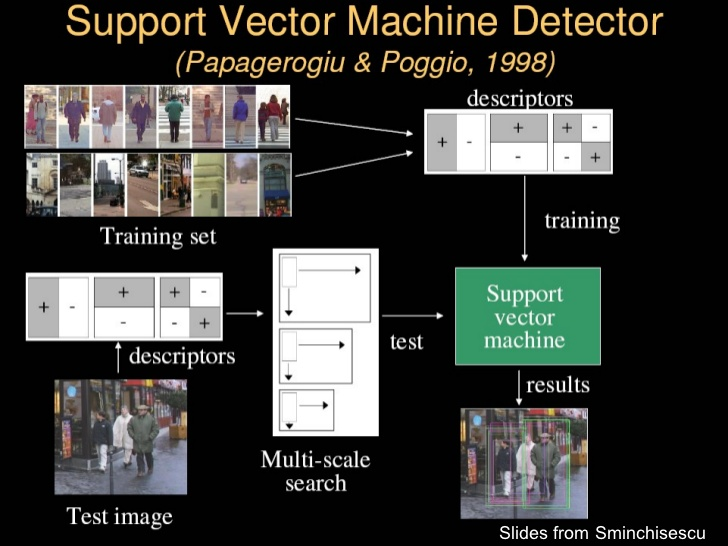
\includegraphics[clip=true,trim= 10 0 80 80,width=0.7\textwidth]{img/hog_svm.jpg}
	    \caption{Illustration HOG+SVM}
   	    \label{fig:hog_topo}
\end{figure}

%%%%%%%%%%%%%%%%%%%%%%%%%%
\subsubsection{Descripteur HOG}
Dans cette méthode, le descripteur (nommé HOG-D) est basé sur un ensemble d'histogrammes de gradient orientés. Les différentes étapes nécessaires au calcul de ces histogrammes est décris ci-dessous:
\paragraph{Découpage de l'image}~\\
\\
Le descripteur est calculé pour une image de 64x128 pixels, ces dimensions représentent les proportions choisi pour une personne. C'est également la résolution utilisée pour la base d'image ``INRIA Person Dataset'' réunie pour tester cette méthode.\\
Cette image est découpée en cellules de 8x8 pixels, ces cellules sont utilisées pour faire des blocs de 2x2 cellules (16x16 pixels). Les blocs se recoupent à 50\%, ce qui donne un total de 7 blocs en largeur par 15 blocs en hauteur.\\
On a donc au final un total de 105 blocs contenant chacun 4 cellules de 8x8 pixels.
\begin{figure}[!ht]
\centering
\begin{subfigure}{.3\textwidth}
  \centering
  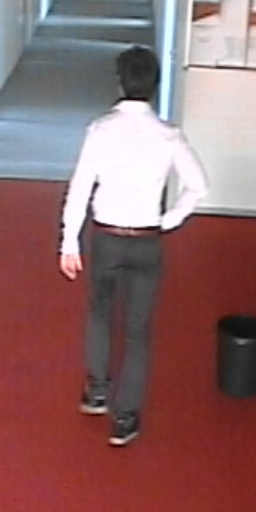
\includegraphics[width=.5\linewidth]{img/person.png}
  \caption{Image d'origine}
  \label{fig:person}
\end{subfigure}%
\begin{subfigure}{.3\textwidth}
  \centering
  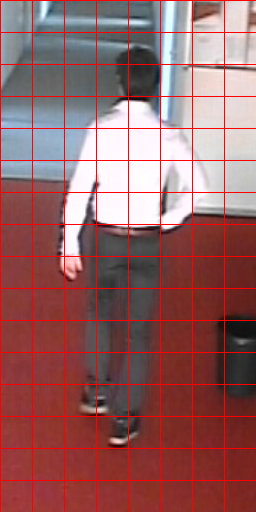
\includegraphics[width=.5\linewidth]{img/cell.png}
  \caption{Découpage en cellules}
  \label{fig:cell}
\end{subfigure}
\begin{subfigure}{.3\textwidth}
  \centering
  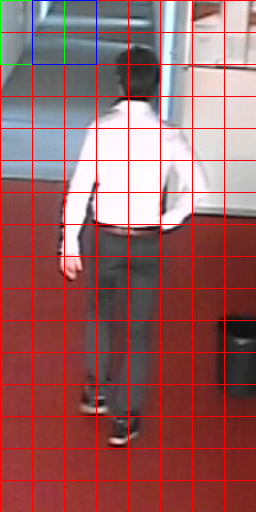
\includegraphics[width=.5\linewidth]{img/block.png}
  \caption{Deux premiers blocs}
  \label{fig:block}
\end{subfigure}
\caption{Découpage de l'image en blocs et en cellules}
\label{fig:decoupage}
\end{figure}
\paragraph{Calcul des gradients}~\\
\\
Les gradients orientés sont calculés à l'aide de deux gradients pour chaque pixel: un gradient horizontal et un gradient vertical notés $S_{x}$ et $S_{y}$ tel que:
\[S_{x(i,j)}=I_{(i+1,j)}-I_{(i-1,j)}\]
\[S_{y(i,j)}=I_{(i,j+1)}-I_{(i,j-1)}\]
Les noyaux utilisés pour calculer ces deux valeurs sont illustrés dans la figure~\ref{fig:kernels}
\begin{figure}[!ht]
\centering
\begin{subfigure}{.3\textwidth}
  \centering
  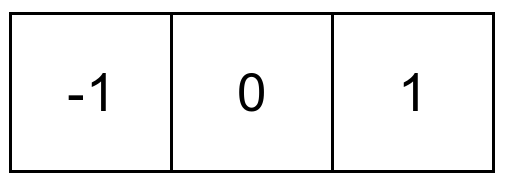
\includegraphics[width=.45\linewidth]{img/Sx.png}
  \caption{$Sx$}
  \label{fig:kernel_sx}
\end{subfigure}
\begin{subfigure}{.3\textwidth}
  \centering
  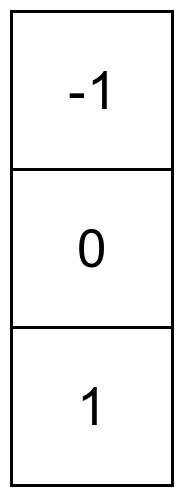
\includegraphics[width=.15\linewidth]{img/Sy.png}
  \caption{$Sy$}
  \label{fig:kernel_sy}
\end{subfigure}
\caption{Noyaux des gradients horizontaux (a) et verticaux (b)}
\label{fig:kernels}
\end{figure}
\\
Le gradient orienté est représenté par le vecteur: $\bar{S}=\begin{pmatrix}S_{x}\\S_{y}\end{pmatrix}$.\\
Les caractéristiques du gradient sont donc:
\[\bar{S}:\begin{cases}
\|S\|=\sqrt{S_{x}^{~2}+S_{y}^{~2}}\\
\Omega_{S} = arctan(\frac{S_{y}}{S_{x}})
\end{cases}\]
\paragraph{Calcul des histogrammes}~\\
\\
Pour chaque cellule, un histogramme est obtenue grâce à la somme pondérée des orientations des gradients. Cet histogramme est réalisé pour 9 valeurs d'orientation par pas de 20\degree les orientations vont donc de 0\degree~à 180\degree.
\begin{figure}[!ht]
    \label{fig:orientations}
    \centering
	    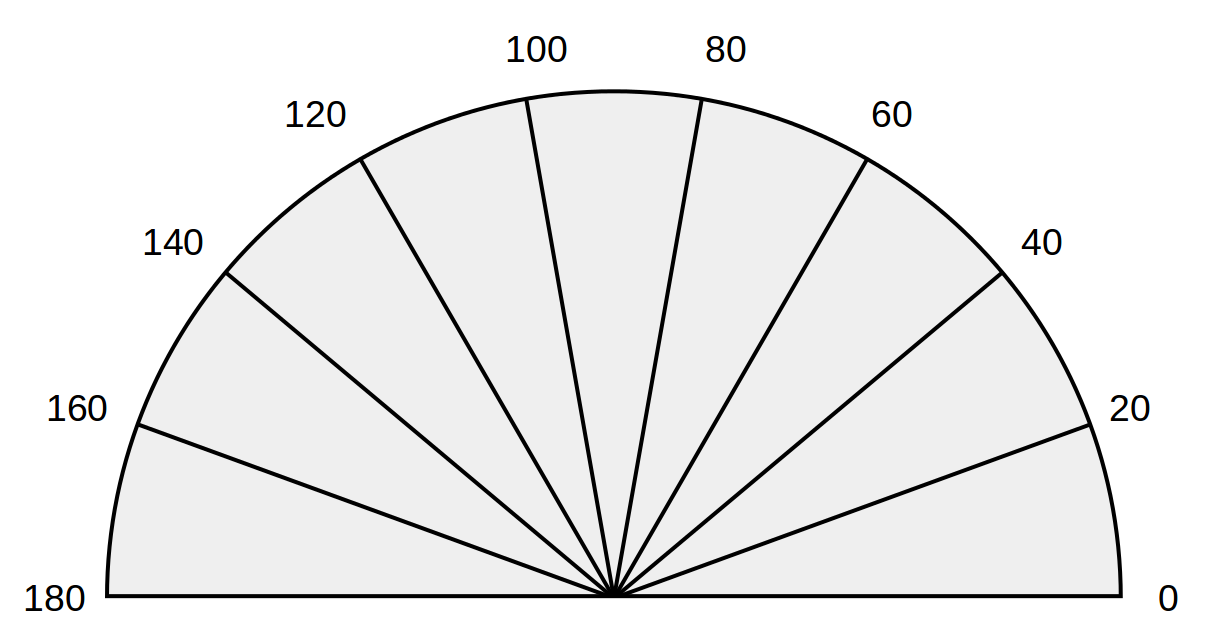
\includegraphics[width=0.5\textwidth]{img/angles.png}
	    \caption{Découpage des orientations des gradients en 9 sections}
\end{figure}
\\
Les centres de ces intervalles sont donc [10;30;50;70;90;110;130;150;170]\degree.
\begin{figure}[!ht]
    \label{fig:histo}
    \centering
	    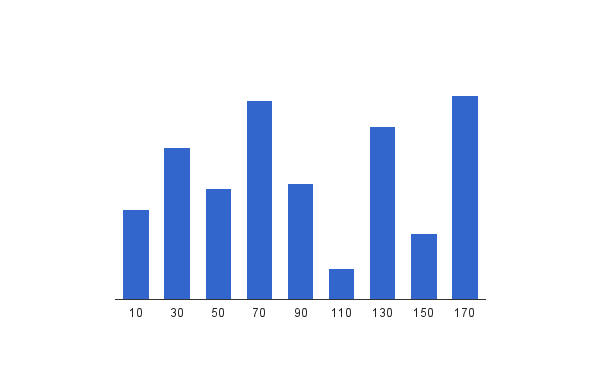
\includegraphics[width=0.5\textwidth]{img/histo.png}
	    \caption{Histogramme obtenu avec centres des intervalles}
\end{figure}
\\
Un gradient ayant pour orientation 50\degree~verra donc son poids (sa norme) ajouté à la barre [40;60]\degree~de l'histogramme de sa cellule.
Les gradients dont l'orientation se situe entre deux centres d'intervalles ont leur poids repartis entre les deux segments de l'histogramme par un principe d'interpolation trilinéaire.\\
\\
Ainsi, si on prend un gradient $\bar{X}$, de norme $\|X\|$ et d'orientation $\theta_{X}=55\degree$, son poids ($\|X\|$) sera reparti entre les segments [40;60]\degree~et [60;80]\degree~de l'histogramme ayant pour centres 50\degree~et 70\degree~respectivement.
Si on note les poids assignés aux deux segments $P_{X50}$ et $P_{X70}$, on obtient:
\[
\begin{cases}
P_{50}(X)=\left ( 1-\frac{|\theta_{X}-50|}{20} \right )*\|X\| = \frac{3}{4}*\|X\|\\
P_{70}(X)=\left ( 1-\frac{|\theta_{X}-70|}{20} \right )*\|X\| = \frac{1}{4}*\|X\|
\end{cases}
\]
Cela permet d'éviter qu'un gradient avec une norme importante se situant à la limite entre deux sections de l'histogramme puisse faire varier le résultat de manière trop importante.
\paragraph{Concaténation et normalisation}~\\
\\
Une fois les histogrammes des quatre cellules d'un bloc calculés, ils sont concaténés afin de former un vecteur de 36 valeurs (4*9).\\
\\
Afin de diminuer l'impact des variations de contraste locales, les histogrammes des blocs sont tous normalisé en divisant leurs valeurs par la norme du vecteur obtenue. On a ainsi un descripteur invariant par rapport au contraste local (bloc de 32x32 pixels) ainsi que par rapport à la luminosité de l'image (caractéristique inhérente aux gradients).
Une fois les histogrammes des blocs sont à leur tour concaténés pour obtenir l'histogramme final.\\
\\
Le descripteur HOG-D nous donne donc vecteur de 3780 valeurs (105 blocs * 36 valeurs) pour représenter une image de 128x64 pixels.
\subsubsection{Classifieur}
Ce descripteur va être utilisé avec un classifieur afin d'effectuer notre détection de personne. Le classifieur utilisé ici est le même que celui utilisé par Dalal et Bill Triggs, une machine à vecteurs de support linéaire (\textit{linear SVM}) entrainée à l'aide de \textit{SVMLight}.
\paragraph{Classification}~\\
\\
Le principe d'un classifieur linéaire est, à l'aide d’exemples positifs et négatifs, de déterminer un hyperplan permettant de séparer l'espace des positifs et celui des négatifs. Un exemple d'ensemble de points positifs et négatifs dans un espace en deux dimensions est présenté en figure~\ref{fig:trainingexamples}.
\begin{figure}[!ht]
    \centering
	    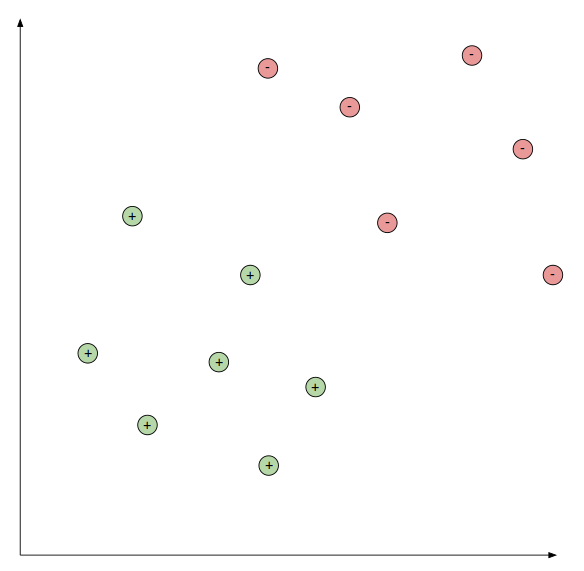
\includegraphics[width=0.35\textwidth]{img/trainingexamples.png}
	    \caption{Exemples positifs et négatifs utilisés pour entrainer la SVM dans un espace 2D}
        \label{fig:trainingexamples}
\end{figure}
\\\\
La particularité de la SVM est d'avoir pour but de trouver l'hyperplan le plus distant des exemples négatifs et positifs. C'est le principe de la route la plus large, on cherche à trouver la route la plus large pouvant séparer les exemples, et une fois définie, l'hyperplan choisi est au centre de la ``route''.\\
Ce principe est illustré dans les figures~\ref{fig:multipleplans} et~\ref{fig:wideststreet}.
\begin{figure}[!ht]
\centering
\begin{minipage}{.5\textwidth}
  \centering
  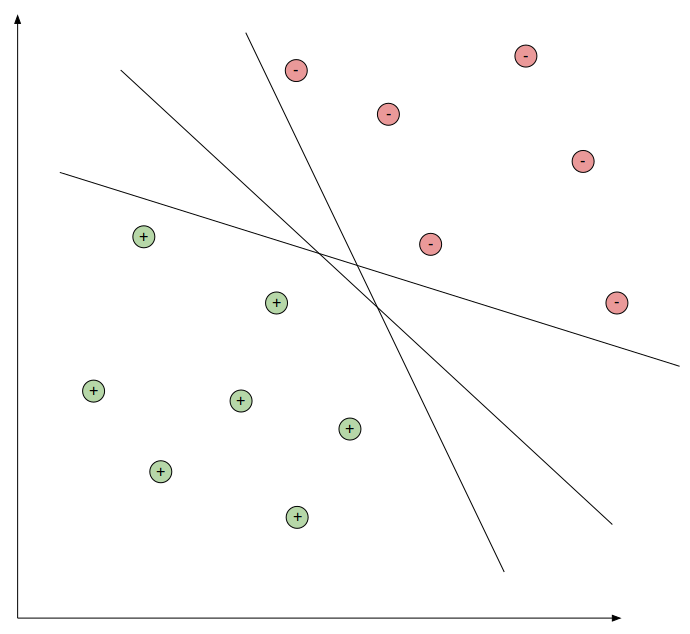
\includegraphics[width=.8\linewidth]{img/multipleplans.png}
  \captionof{figure}{Différents hyperplans valides}
  \label{fig:multipleplans}
\end{minipage}%
\begin{minipage}{.5\textwidth}
  \centering
  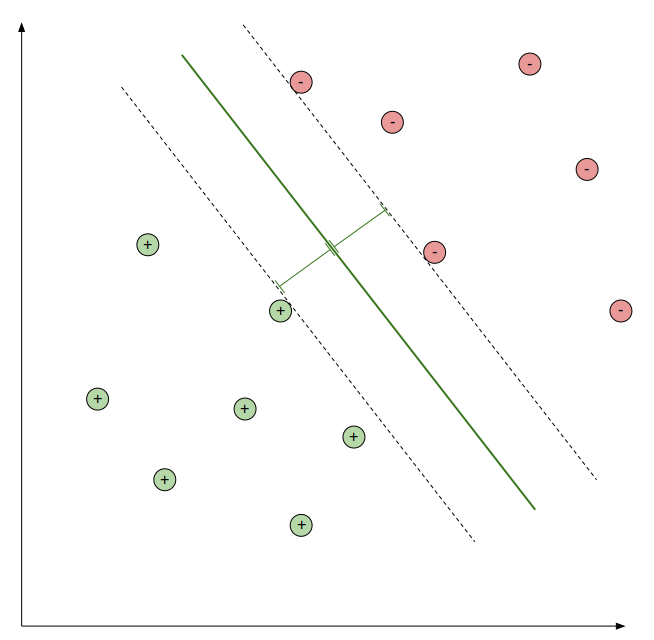
\includegraphics[width=.8\linewidth]{img/wideststreet.png}
  \captionof{figure}{Hyperplan avec la marge la plus large}
  \label{fig:wideststreet}
\end{minipage}
\end{figure}
\\
\\
Une fois l'hyperplan défini lors de l'entrainement de la SVM avec des exemples positifs et négatifs, on peut s'en servir pour déterminer si un point donné dans cet espace est positif ou non selon sa position par rapport à l'hyperplan.\\
Pour cela, on utilise un vecteur unitaire normal à l'hyperplan sur lequel on projette le vecteur des paramètre du point expérimental, la valeur de cette projection est comparée avec celle déterminée par l'hyperplan.
\begin{figure}[!ht]
    \centering
	    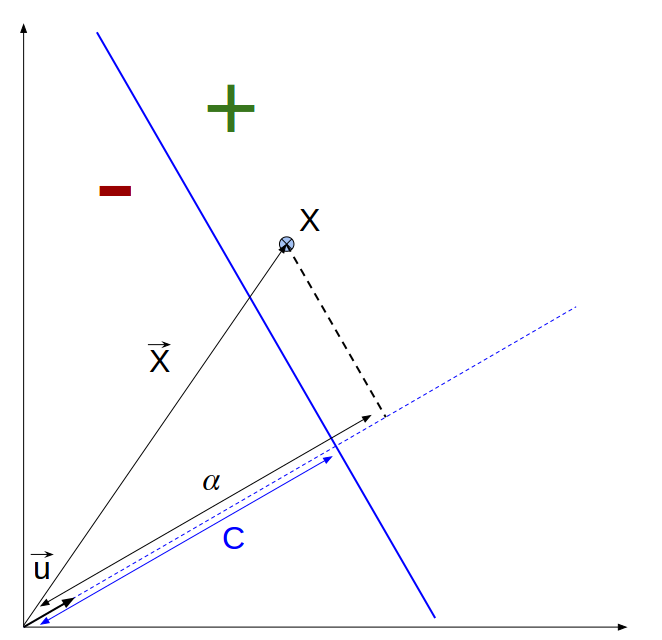
\includegraphics[width=0.4\textwidth]{img/projection.png}
	    \caption{Utilisation de l'hyperplan pour classifier un exemple X}
        \label{fig:projection}
\end{figure}
\\
Si on note la distance entre l'origine et l'hyperplan $C$, $\bar{w}$ le vecteur unitaire normal à l'hyperplan, et $\bar{X}$ le point expérimental à classifier, on a la relation suivante:
\[\alpha=\bar{X}\cdot\bar{u}~
\begin{cases}
\alpha\geq C\rightarrow~$cas positif$\\
\alpha<C\rightarrow~$cas négatif$
\end{cases}
\]
\paragraph{Fenêtre glissante multi-échelle et suppression des non-maxima}~\\
\\
Une fois la SVM entrainée, on peut utiliser une fenêtre glissante le long d'une image afin de déterminer les parties de l'images classifiées comme des personnes. Pour pouvoir détecter les personnes de différentes tailles et à différentes distances on repasse la fenêtre à différentes échelles.\\
\\
On a alors une liste des sous-rectangles de l'images contenant une personne, le problème étant qu'une même personne peut être détectée dans plusieurs rectangles de tailles et de positions légèrement différentes et on obtient une multitudes de rectangles positifs pour une seule personne.\\
Afin de résoudre ce problème, on utilise un algorithme de suppression des non-maxima sur l'ensemble des rectangles obtenus.\\\\
Le principe est de mesurer la similitude entre deux rectangle, notée $\epsilon$, en fonction de leurs tailles et positions, au delà d'un certain seuil paramétrable, les deux rectangles similaires sont réunis.\\
On peut également choisir un seuil pour le nombre minimum de rectangles dans un cluster pour que la détection soit gardée, et enfin tout les rectangles étant inclus dans des rectangles plus grand avec plus d’occurrences sont également supprimés.\\
Le résultat cet algorithme une fois paramétré est illustré dans la figure~\ref{fig:nonmaxima}.
\begin{figure}[!ht]
	\centering
	\begin{subfigure}{.45\textwidth}
		\centering
		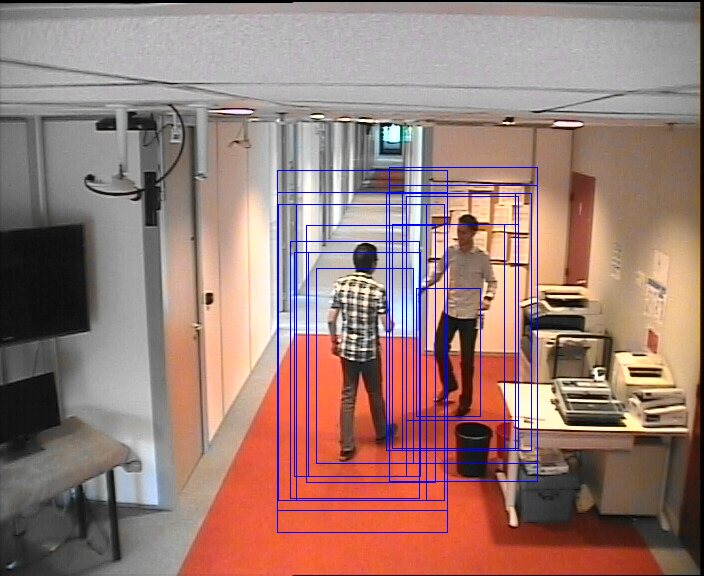
\includegraphics[clip=true,trim=200 0 100 100,width=\linewidth]{img/nonmax1.png}
		\caption{Résultat de HOG-D+SVM linéaire}
	\end{subfigure}
	\begin{subfigure}{.45\textwidth}
		\centering
		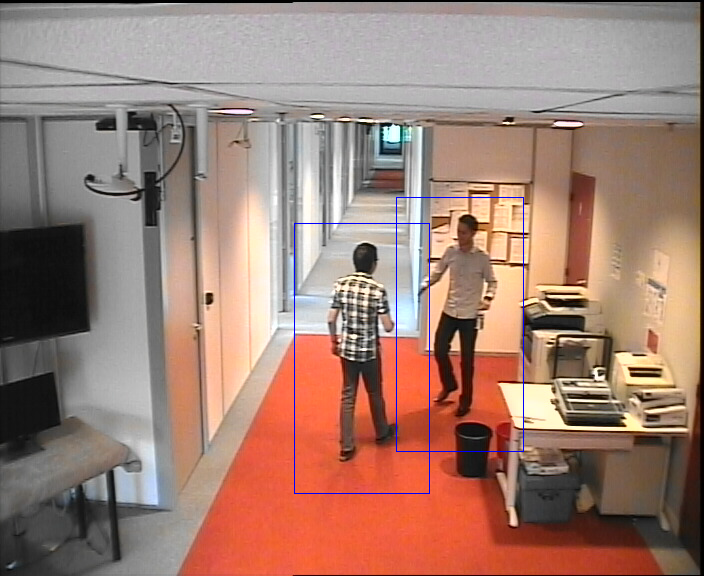
\includegraphics[clip=true,trim=200 0 100 100,width=\linewidth]{img/nonmax2.png}
		\caption{Suppression des non-maxima}
	\end{subfigure}
	\caption{Algorithme de suppression des non-maxima}
	\label{fig:nonmaxima}
\end{figure}
\subsubsection{Paramétrage et résultats}
Une fois la méthode de détection et son implémentation choisis, il reste à en régler les paramètres afin de correspondre à nos besoins.\\
Dans un cadre de suivi de personnes, le but est d'avoir un bon taux de détection mais surtout de minimiser les faux positifs. En effet, ne pas détecter un personne est pénalisant, mais si on détecte un faux positifs et qu'on zoom dessus, on perd énormément de temps, et ce temps perdu est plus pénalisant que de perdre une personne. Avec les contraintes physiques de la caméra et notamment les délais importants pour zoomer et dé-zoomer, la priorité est d'être certain d'avoir détecter une personne.\\
Notre ``cahier des charges'' de détection est donc le suivant:
\begin{itemize}  
	\item environnement temps réel: un minimum de 5 images par secondes; 
	\item taux de faux positifs proche de 0;
	\item taux de détection le plus haut possible en respectant les deux premières contraintes.
\end{itemize}
Afin d'atteindre notre but, on peut jouer sur plusieurs paramètres dans l'algorithme de détection.\\
\\
Le premier paramètre, qui influe le plus sur le temps de détection est la plus petite taille de fenêtre utilisée pour parcourir l'image et l'échelle de multiplication entre deux tailles de fenêtres.\\
La taille minimum de fenêtre est fixée sur une fenêtre de 8x16 pixels, l'algorithme n'étant pas fiable pour des images plus petites.\\
L'échelle est déterminée comme un compromis en rapidité et robustesse de détection, une échelle de 1.15 nous donne de bon résultats en détection (plusieurs fenêtres positives pour une personne), et nous permet d'obtenir une vitesse de calcul entre 60 et 70 millisecondes soit environ 15 images par seconde pour la seule détection. L'effet de l'échelle est illustrée dans la figure~\ref{fig:multiscale}.
\begin{figure}[!ht]
	\centering
	\begin{subfigure}{.25\textwidth}
		\centering
		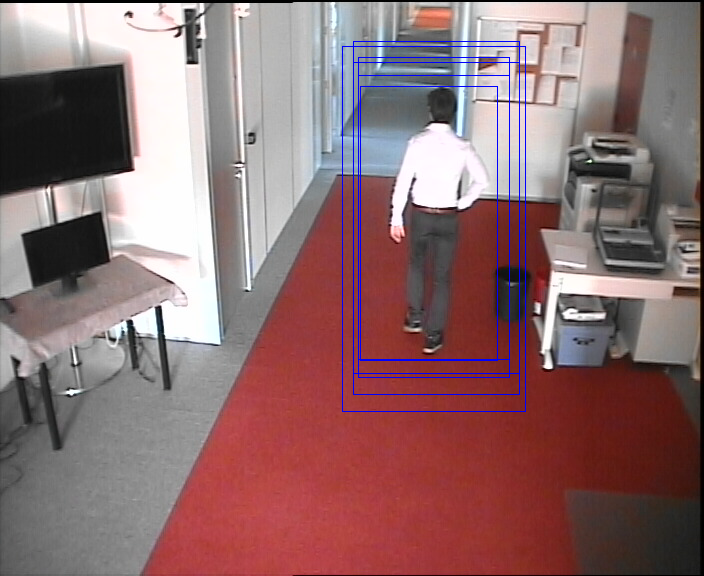
\includegraphics[clip=true,trim=300 100 150 0,width=\linewidth]{img/multiscale11.png}
		\caption{Échelle de 1.1}
	\end{subfigure}
	\begin{subfigure}{.25\textwidth}
		\centering
		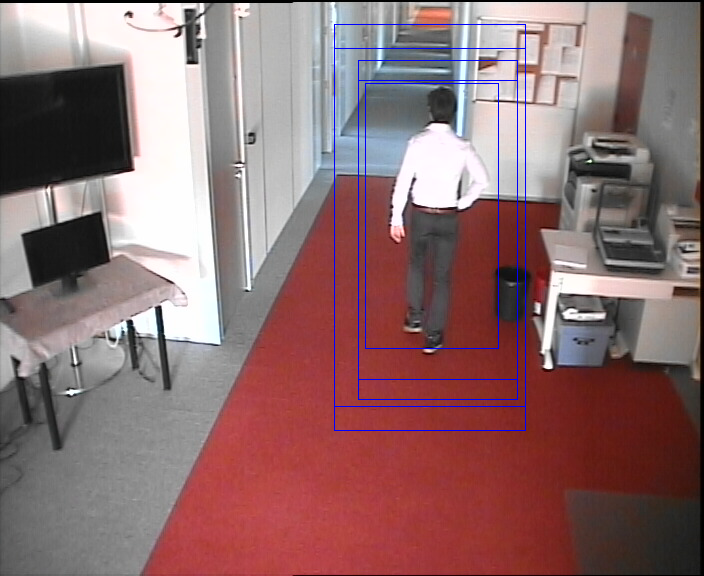
\includegraphics[clip=true,trim=300 100 150 0,width=\linewidth]{img/multiscale12.png}
		\caption{Échelle de 1.2}
	\end{subfigure}
	\begin{subfigure}{.25\textwidth}
		\centering
		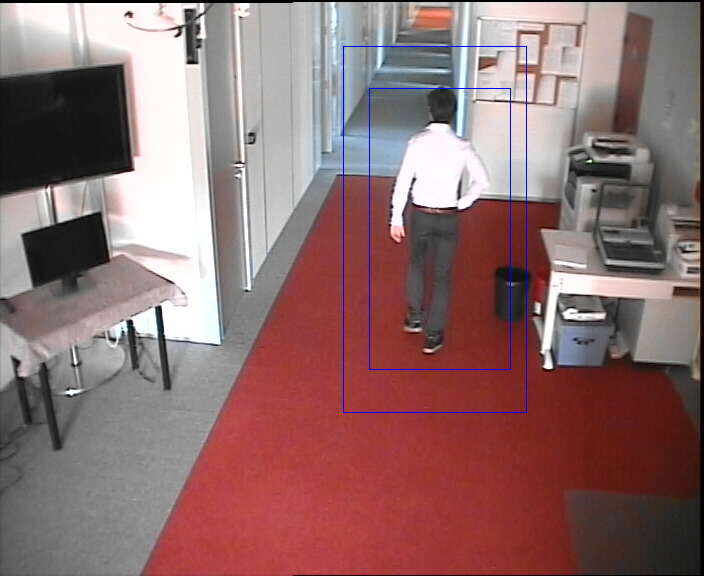
\includegraphics[clip=true,trim=300 100 150 0,width=\linewidth]{img/multiscale13.png}
		\caption{Échelle de 1.3}
	\end{subfigure}
	\caption{Influence de l'échelle de taille pour les fenêtres de détection}
	\label{fig:multiscale}
\end{figure}\\
\\
Ce temps de calcul nous laisse une marge confortable pour les différents calculs nécessaires au suivi de personnes. La détection étant la partie nécessitant le plus de temps de calcul, on peut s'attendre un système final capable de fonctionner à plus de 10 images par secondes, ce qui est satisfaisant pour notre cas.\\
\\
Le second paramètre est le seuil à partir duquel une fenêtre est considérée comme une détection positive, l'équation précédente devient en pratique $\alpha\geq~C+\tau$ avec $\tau$ le seuil choisi. L'effet du seuil est illustrée dans la figure~\ref{fig:seuil}.
\begin{figure}[!ht]
	\centering
	\begin{subfigure}{.45\textwidth}
		\centering
		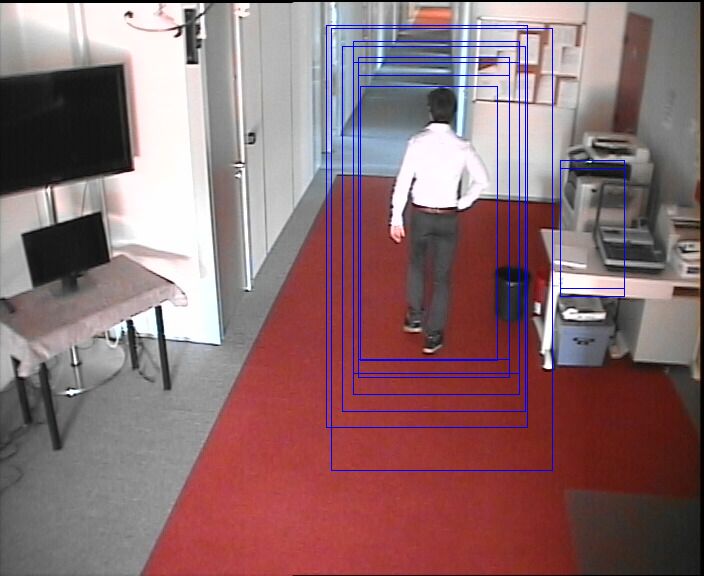
\includegraphics[clip=true,trim=300 100 50 0,width=\linewidth]{img/tau0.png}
		\caption{$\tau=0$}
	\end{subfigure}
	\begin{subfigure}{.45\textwidth}
		\centering
		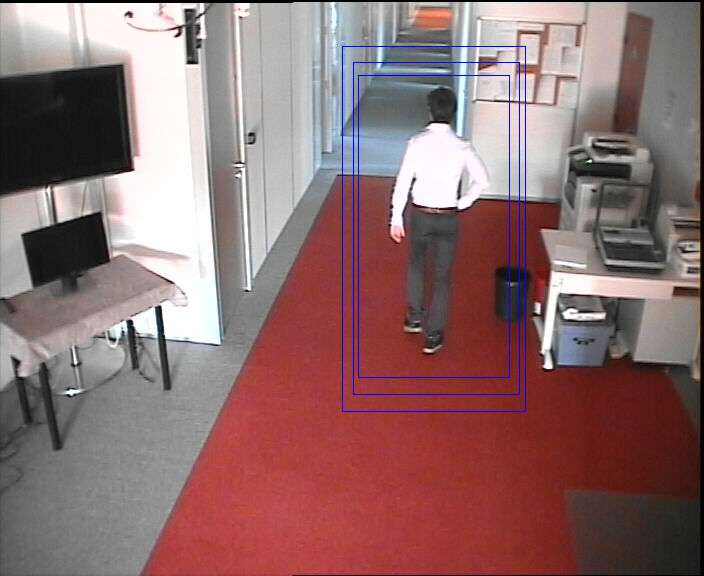
\includegraphics[clip=true,trim=300 100 50 0,width=\linewidth]{img/tau1.png}
		\caption{$\tau=1$}
	\end{subfigure}
	\caption{Influence du seuil de détection}
	\label{fig:seuil}
\end{figure}\\
\\
Ce seuil n'influence pas le temps de calcul de l'algorithme, c'est donc un compromis entre le taux de détection et le taux de faux positifs. \\Notre priorité étant d'avoir très peu de faux positifs, le seuil a été mis à une valeur $\tau=0.35$ permettant de supprimer pratiquement tout les faux positifs dans notre environnement de test.
\subsubsection{Implémenation}
La détection est implémentée sous la forme d'une classe \verb!detector! dont la déclaration est présentée ci-dessous.\\
\begin{lstlisting}[frame=single]
class detector{
public:
  detector(float threshold=0, float scale=1.05, float recTh=2);
  void detection(cv::Mat &frame,std::vector<cv::Rect> &det);
private:
  cv::HOGDescriptor hogD;  //descriptor	
  float threshold;	   //detection threshold	
  float scale;		   //windows scaling	
  float recTh;		   //non-maxima supression threshold
};
\end{lstlisting}
Le constructeur permet de régler les paramètres du classifieur et d'initialiser le détecteur avec le descripteur HOG-D entrainé sur les personnes.\\
Ces paramètres sont stockés dans la classe et seront utilisés lors de l'appel de la fonction \verb!detection()! qui prend en argument l'image sur laquelle effectuer la détection (\verb!frame!) et le vecteur de rectangles dans lequel sera stocké les détections (\verb!det!).\\
\\
Cette fonction \verb!detection()! applique la détection multi-échelle, et l'algorithme de suppression des non-maxima, et ajoute les rectangles obtenues dans le vecteur de rectangle \verb!det!.
\subsubsection{Résultats}
Après réglage des paramètres de l'algorithme, on obtient un détecteur nous permettant d'avoir un taux de faux positifs pratiquement nuls et un très bon taux de détection pour les personnes de face et de dos.\\
Pour des personnes représentés par plus de 50 pixels en hauteur, la détection est presque parfaite, la personne n'est que très rarement non-détectée, et ces pertes de détections seront gérées au niveau supérieur par le suivi.\\
Les personnes de profils ont un taux de détection légèrement plus variable, mais avoisinant les 80 à 90\% lors des tests, ce qui est également suffisant pour le suivi.\\
\\
Les faux positifs sont très rares, et éliminés au niveau supérieur également, toute détection intermittente étant filtrée par le suivi qui sélectionne les détections avec une certaine constance.\\
\\
On a donc un système de détection robuste, ce qui nous permet d'avoir de bonnes bases pour construire notre système d'identification et de suivi des personnes.
\pagebreak
\subsection{Identification des personnes}
Le but est d'acquérir des informations sur chaque personne passant dans le champs de vision de la caméra, pour ça il est nécessaire de zoomer sur chacune afin d'obtenir une image plus détaillée.
Si possible (personne de face), on peut également faire une détection du visage et zoomer encore plus afin d'acquérir des images suffisament haute résolution pour une future reconnaissance.\\
\\
Cette opération de zoom/acquisition est relativement simple une fois une personne détectée (il suffit de régler le niveau de zoom de la caméra et les angles \textit{pan} et \textit{tilt}). complexity arise when deux personnes ou plus sont dans le champ de cette caméra.\\
Il faut alors mettre en place une méthode d'identification des personnes et un moyen de décider sur quelle personne effectuer cette acquisition. Une fois l'acquisition effectuée, il sera aussi nécessaire de pouvoir ré-identifier les personnes présentes dans l'image afin de ne pas effectuer l'action deux fois sur la même personne.\\
\\
Le but est donc d'avoir un système capable de différencier les personnes présentes dans une image, de décider sur quelle personne se concentrer en priorité, et après un zoom/dé-zoom sur cette personne, de ré-identifier les personnes présentes dans l'image.

\end{document}